The sole purpose of this layer is to control the Turning Board. This layer is directly accessible to the user. This remote is in the form of an android app or IOS app. This layer communicates with the Main Control layer adequately to propagate user commands. Some features included in this layer include: user authentication, and user ride data analysis.

% is controlled directly by the user. It takes the form of an app that sends data to the Main Control layer for the appropriate signals to be sent to the other layers. The app requires an authentication process to log into it. It will also provide the user with ride data analysis after a trip on the board is completed.This app is available on iOS and Android.

\subsection{Front-end UI and Main Control communication }
The front-end UI and the Main Control layer, currently, communicate via internet. With a Firebase back-end set up, the UI interfaces with the back-end, which in turn propagates data to the Main Control. The back-end the system is using consists of a real-time NoSQL database. The Main Control, in turn, retrieves the appropriate data and passes it on to the corresponding subsystem.


\begin{figure}[h!]
	\centering
 	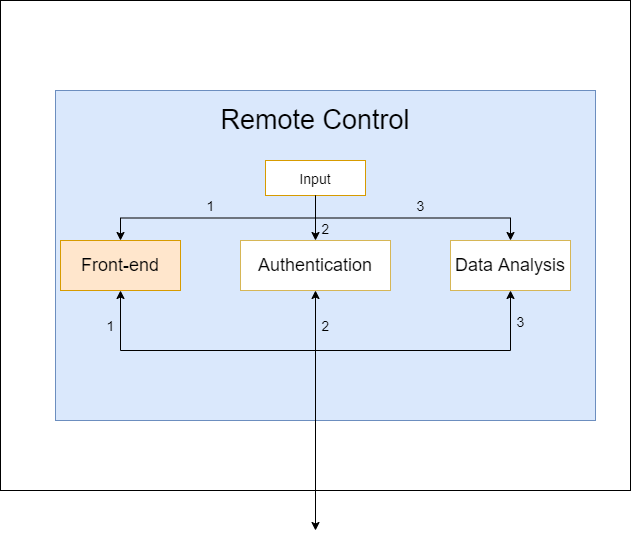
\includegraphics[width=0.60\textwidth]{DDS/images/UIJetsonCom.png}
 \caption{Example subsystem description diagram}
\end{figure}

\subsubsection{Assumptions}
It is assumed that the latency between data posting by the front-end and data retrieval by the Main Control is almost negligible. It is also assumed the user is always connected to the internet while the Turing board is active.

\subsubsection{Responsibilities}
The UI must present the user with an easy to user interface. The UI must the post the component's data to a real-time database as soon as the state of a component changes.

\subsubsection{Subsystem Interfaces}
Each of the inputs and outputs for the subsystem are defined here.
\begin {table}[H]
\caption {Subsystem interfaces} 
\begin{center}
    \begin{tabular}{ | p{1cm} | p{6cm} | p{3cm} | p{3cm} |}
    \hline
    ID & Description & Inputs & Outputs \\ \hline
    \#1 & Giving the UI a command & \pbox{3cm}{User command} & \pbox{3cm}{raw data to a database}  \\ \hline
    \end{tabular}
\end{center}
\end{table}

\subsection{Authentication}
When the user attempt to log into the app or sign up, the UI parses the login/signup information (name, email, password, etc.) the parsed data is then sent to a Firebase authentification API. The API in turn forwards a token to the app confirming status of the attempt, either successful or unsuccessful login/sign up. The app then uses the data to render the UI accordingly.

\begin{figure}[h!]
	\centering
 	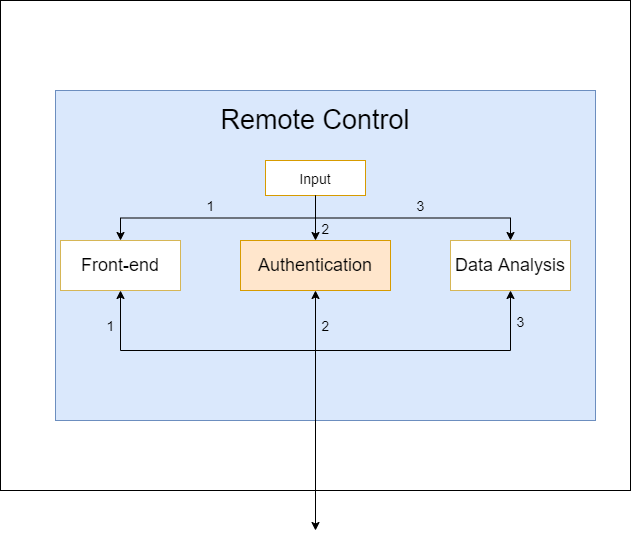
\includegraphics[width=0.60\textwidth]{DDS/images/Authentication.png}
 \caption{Example subsystem description diagram}
\end{figure}

\subsubsection{Responsibilities}
This feature makes sure a user has access to the UI controller or not. It makes sure the right data will be sent to the right Turing board.

\subsubsection{Subsystem Interfaces}
Each of the inputs and outputs for the subsystem are defined here.
\begin {table}[H]
\caption {Subsystem interfaces} 
\begin{center}
    \begin{tabular}{ | p{1cm} | p{6cm} | p{3cm} | p{3cm} |}
    \hline
    ID &  \\ \hline
    \#1 & Authentication & \pbox{3cm}{user information} & \pbox{3cm}{un/successful token}  \\ \hline
    \end{tabular}
\end{center}
\end{table}

\subsection{Ride Data Analysis}
This will be information provided to the user after a ride. This information may include average speed of the ride, the duration of the ride, and the distance traveled.

\begin{figure}[h!]
	\centering
 	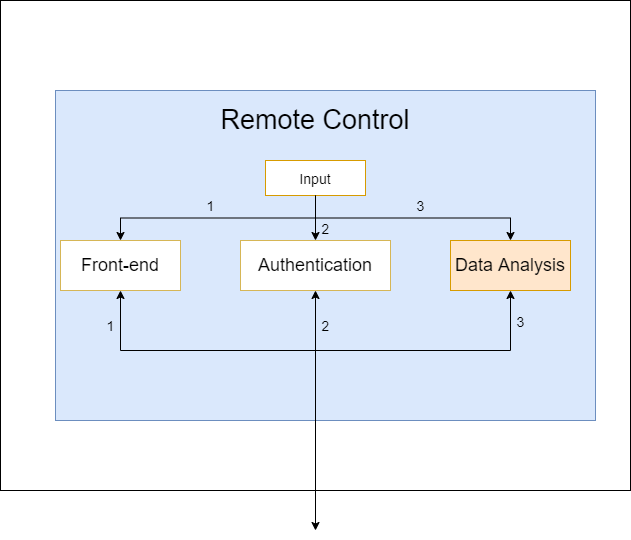
\includegraphics[width=0.60\textwidth]{DDS/images/dataAnalysis.png}
 \caption{Example subsystem description diagram}
\end{figure}

\subsubsection{Responsibilities}
Provide users with their ride analysis.

\subsubsection{Subsystem Interfaces}
Each of the inputs and outputs for the subsystem are defined here.
\begin {table}[H]
\caption {Subsystem interfaces} 
\begin{center}
    \begin{tabular}{ | p{1cm} | p{6cm} | p{3cm} | p{3cm} |}
    \hline
    ID & Description & Inputs & Outputs \\ \hline
    \#1 & Ride analysis & \pbox{3cm}{refined database data} & \pbox{3cm}{legible ride analysis data}  \\ \hline
    \end{tabular}
\end{center}
\end{table}


